\chapter{Komponenty rękawicy-kontrolera}
\label{ch:komponenty}
Wspomniane były do tej pory projekty komercyjnych rękawic-kontrolerów, jednak w celu dokładnego działania, wykorzystują one złożone techniki w celu osiągnięcia jak najlepszych rezultatów, jak i również dodatkowe moduły pozwalające na rozwiązanie problemów w bardziej wyszukany sposób - często poprzez analizę otoczenia, bądź gdy "otoczenie" analizuje gdzie znajduje się kontroler. W przypadku podstawowej wersji nie użyto żadnych dodatkowych systemów a jedynym zamiarem jest wykorzystanie podstawowych, łatwo dostępnych bądź możliwych do skonstruowania elementów w celu rozwiązania problemów nawigacji inercyjnej. W związku z tym najpierw zdefiniowano czym jest nawigacja inercyjna.N awigacja inercyjna, znana również pod akronimem INS(z ang. Inertial Navigation System), jest to dziedzina problemowa która zawiera metody określanie pozycji przy użyciu sensorów wykorzystujących zasady działania fizyki. Sensory te to akcelerometr oraz żyroskop. Akcelerometr dzięki wykorzystaniu drugiej zasady dynami Newtona, pozwala określić oddziaływanie siły na urządzenie na podstawie sił jakie oddziałują na niego samego. Żyroskop natomiast uzyskuje pomiar działania prędkości kątowych dzięki czemu jest w stanie określić orientację urządzenia. Dzięki wykorzystaniu tych sensorów, w teorii jesteśmy w stanie określić dokładne położenie i orientację bez konieczności użycia zewnętrznego źródła pomiarów. Warto zauważyć że jest tak tylko w teorii ponieważ w praktyce sensory te podlegają wielu błędom przez które niemożliwym jest określenie położenia w przestrzeni z wystarczającą dokładnością aby oszukać zmysły człowieka w szczególności w systemach wirtualnej rzeczywistości~\cite{podstawy}.
		
	\section{IMU - Inercyjna jednostka pomiarowa}
	\label{sec:imu}
	Aby można było stosować pomiar w ramach nawigacji inercyjnej zostały stworzone inercyjne jednostki pomiarowe, znane jako IMU(z ang. Inertial Measurement Unit), które w podstawowej wersji występują w postaci połączenia akcelerometru oraz żyroskopu. W wersji bardziej zaawansowanej dołączony jest również trzy osiowy magnetometr i w popularnych produktach rękawic to właśnie ten rodzaj IMU jest najczęściej spotykany. W celu lepszego zrozumienia działania tej jednostki zostaną przedstawione kolejno sensory wchodzące w jego skład oraz zostanie wyjaśnione pojęcie wieloosiowego pomiaru, które jest bezpośrednio powiązane z określeniem stopni swobody~\cite{bSensory}.
		\subsection{Sensory}
		\label{subsec:sensory}
		Akcelerometr jest prostym sensorem którego budowa opiera się o zamocowanie małej masy na sprężynach które ją utrzymują. W zależności od tego jak zadziała siła na akcelerometr sprężyna wyciągnie się bądź skurczy, wprawiając ciało w ruch. Masa ta jest częścią układu kondensatora pomiarowego, co oznacza że w wyniku poruszania zmienia się jego pojemność - czyli napięcie wyjściowe. Napięcie to dalej jest przekazywane do mikroprocesora bądź przetwornika analogowo-cyfrowego, a wynik podawany jest w {\Large$\frac{m}{s^2}$}. Sensor ten głównie jest wykorzystywany do pomiaru przemieszczenia. Drugim równie ważnym sensorem którego celem jest pomiar prędkości kątowej jest żyroskop. Żyroskop wykorzystuje do działania zjawisko znane jako efekt Coriolisa. Polega ono na wytwarzaniu siły prostopadłej do masy, umieszczonej na talerzu żyroskopu, która przemieszcza się względem zadanej osi. Przemieszczanie się tej masy jest mierzone przy użyciu kondensatorów. Oznacza to że siła ta mierzona jest tylko gdy sensor podlega rotacji, wprawiając masę znajdującą się w środku w ruch - w przypadku gdy sensor jest w pozycji stacjonarnej, niezależnie od aktualnej rotacji, odczyty wskazują zero na wszystkich osiach pomiaru. Jednostką pomiaru są {\Large $\frac{rad}{s}$}, co oznacza że uzyskanie orientacji w postaci kąta obrotu jest możliwe poprzez całkowanie wartości uzyskanych z żyroskopu. Ostatnim czujnikiem wykorzystywanym w IMU jest magnetometr,dzięki któremu uzyskiwana jest wartości pola magnetycznego oraz jego kierunek. Istnieje kilka sposobów na odczyt tych danych w związku z czym metody budowy magnetometru nie zostaną w tej pracy opisane. Magnetometru używa się w celu określenia kierunku magnetycznego bieguna północnego ziemi. Aby osiągnąć geograficzny kierunek bieguna północnego należy do tej wartości dodać deklinację geograficzną która rożni się w zależności od miejsca na ziemi w którym znajduje się magnetometr. Magnetometr zwraca wartości podane w mikro-Teslach zapisywanych jako $\mu T$. Tak jak pozostałe sensory również ten jest wrażliwy na zaburzenia odczytów. W przypadku magnetometru są to pola magnetyczne wokół których znajduje się sensor~\cite{bSensory}.
		\subsection{Stopnie swobody}
		\label{subsec:swobody}	
		Do tej pory powiedziano o działaniu sensorów przy których stwierdzono że działają one wokół pewnych osi. Świat trójwymiarowy jest reprezentowany jako układ trzech osi ustawionych do siebie prostopadle. Jeżeli sensor nazywany jest trójosiowym, oznacza to że dokonuje on pomiaru we wszystkich kierunkach dzięki czemu jesteśmy w stanie określić dane w przestrzeni trójwymiarowej. W zależności od sensora IMU, dane te pozwalają określić wartości takie jak położenie, orientację w przestrzeni względem punkty początkowego, a gdy ten jest znany orientację bezwzględną, oraz kierunek względem biegunów ziemi. Stopień swobody oznacza możliwość pomiaru danego parametru wokół zadanej osi. W ten oto sposób jeżeli mamy do czynienia z 3-osiowym akcelerometrem oraz 3-osiowym żyroskopem mówimy o 6 stopniach swobody, oznaczanych jako 6DoF (z ang. 6 Degrees of Freedom), czyli położenie względem punktu zero, oznaczonego jako dystans na osi X,Y oraz Z, a także orientację wokół tych osi, opisywanych jako wartość przechylenia, nachylenia oraz zbaczania z trasy. W literaturze jednak powszechnie stosowane są angielskie określenia roll, pitch oraz yaw. Roll jest określany jako obrót wokół osi poziomej wzdłużnej, pitch jest definiowany jako obrót wokół osi poprzecznej modelu, natomiast yaw jako obrót wokół osi pionowej. Rysunek~\ref{fig:rpy} pokazuje umiejscowienie modelu samolotu w punkcie zero układu współrzędnych oraz rotację wokół tych osi reprezentując 6DoF. 
\begin{figure}[h]
\centering
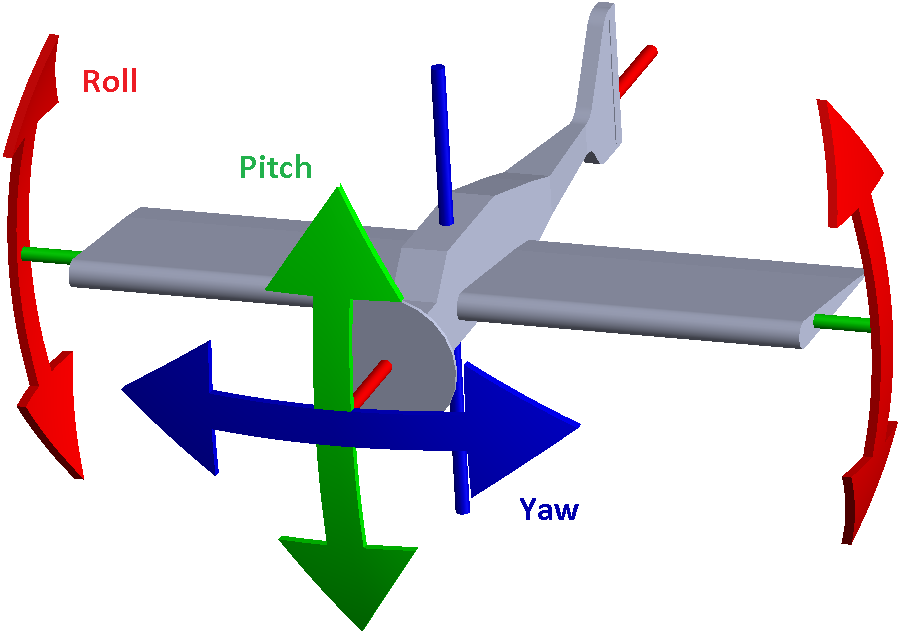
\includegraphics[width = 0.7\textwidth]{RPY}
\captionsource{Model prezentujący sześć stopni swobody}{\url{http://www.rc.info.pl/slownik/roll-pitch-yaw-katy-rpy/}}
\label{fig:rpy}
\end{figure}	
Ten rodzaj ustawienie obrazujący kierunek oraz rotacje, w przestrzeni trójwymiarowej na podstawie trójosiowego układu współrzędnych jest nazywany kątami Tait–Bryan'a. Kąty te jednak mają jedną poważną wadę. W skutek obrotu wokół osi, jest możliwa utrata jednego stopnie swobody. Dzieję się to z powodu rotacji w której dwie z trzech osi żyroskopu zostaną ustawione do siebie równolegle. Spowodowane jest to tym że obrót jest odwzorowywany z danych żyroskopu według jednej osi jednocześnie, co sprawia że kolejność wykonywania rotacji ma znaczenie. Kolejność od pierwszej do ostatniej jest określana jako obrót zewnętrzny, środkowy oraz wewnętrzny. W przypadku kolejności obrotu wokół osi Y, następnie X a ostatecznie Z, jeżeli dokonamy obrotu wokół osi X o $90^o$, sprawi to że oś zewnętrzna Y a także wewnętrzna Z ustawią się w jednej płaszczyźnie, w związku z czym stracimy możliwość obrotu względem jednej osi. Problem ten obrazuje rysunek~\ref{fig:gimbal}. Jeżeli w jednostce używany jest również magnetometr, określa się takie IMU jako 9DoF. Podsumowując - w zależności od użytych sensorów, oraz osi wokół których zostały ustawione sensory, mówimy o odpowiedniej ilości stopni swobody. Oznacza to że jeżeli użyjemy trzech akcelerometrów i żyroskopów, jednak wszystkie będą ustawione wokół tej samej osi mówimy o 2DoF, jeden dla przemieszczenia, drugi dla rotacji wokół tej osi~\cite{rotations}~\cite{botland-arduino}.	
\begin{figure}[h]
\centering
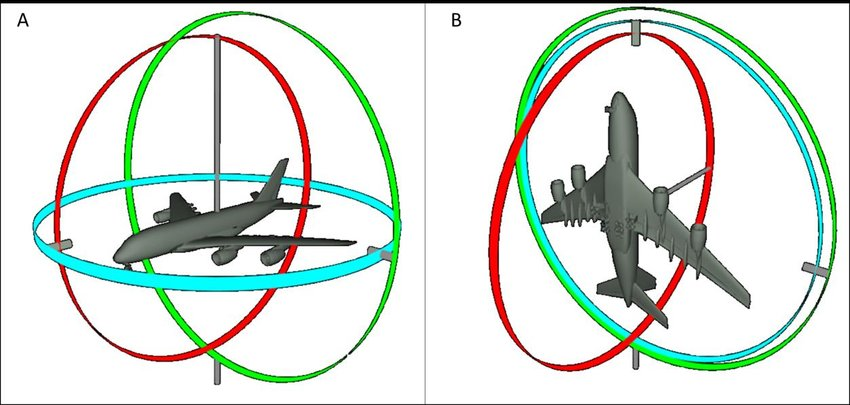
\includegraphics[width = \textwidth]{gimbal}
\captionsource{Problem blokady gimbala (Przed i po obrocie)}{\url{https://www.researchgate.net/figure/Gimbal-lock-problem-for-Euler-angles-A-no-gimbal-lock-B-yaw-and-roll-angles-are_fig14_332394380}}
\label{fig:gimbal}
\end{figure}	
		
\section{Śledzenie położenia palców}
\label{sec:palce}
 Aby mówić o kontrolerze w postaci rękawicy, wymaganym elementem jest możliwość śledzenia położenia palców dłoni. Rozwiązania tego problemu zazwyczaj widuje się w postaci jednego z dwóch sposobów. Pierwszym sposobem jest wykorzystanie wspomnianych IMU i umieszczenie ich na dłoni w cel uzyskania pozycji całej ręki oraz na palcach w celu ich śledzenia. W takim wypadku, w spotkanych rozwiązaniach użyte zostały dwa bądź trzy IMU na każdym z palców. Następnie dane ze wszystkich sensorów, ze wszystkich IMU zostają złożone w całość w celu wygenerowania pozycji każdego z czujników na ekranie użytkownika. Rozwiązanie to jest znacznie bardziej skomplikowane lecz oprócz zginania palców pozwala na określenie ich odwodzenia co zapewnia dużo bardziej realne wrażenia. Rozwiązanie to jednak nie jest tanie, a także sposób integrowania danych jest bardziej skomplikowany. Alternatywą tego rozwiązania jest wykorzystania czujników zgięcia. Czujnik taki umiejscowiony na palcu pozwala na określenie stopnia wygięcia. Rozwiązanie to jest proste w implementacji, jednak czujniki pozwalające na dokładne pomiary również nie są tanie~\cite{flex-sensor}~\cite{manus}.
			
\section{Łączność przy użyciu Bluetooth niskiego poboru mocy}
\label{sec:bvsble}
Ostatnim elementem ważnym dla rękawicy jest możliwość przesyłania danych. Dane można przesyłać w tradycyjny sposób przewodem przy użyciu odpowiednich złączy, jednak w celu większego komfortu użytkowania i spełnienia realizmu wirtualnej rzeczywistości połączenia bezprzewodowe są tymi które dostarczają lepsze wrażenia. Wśród połączeń bezprzewodowych wykorzystywane jest połączenie przy użyciu Bluetooth a w szczególności BLE (z ang. Bluetooth Low Energy). Rozwiązanie to kosztem transferu osiągnęło długi czas pracy na minimalnym zasilaniu, przy czym w wersji 5.0 pozwala również na współpracę z wieloma urządzeniami jednocześnie, co może okazać się przydatne gdy korzystamy z dwóch rękawic jednocześnie. 

Gdy mowa o połączeniu BLE warto znać kilka podstawowych terminów. Przede wszystkim trzeba wiedzieć czym jest GATT (z ang. Generic Attribute Profile). Jest to struktura pozwalająca na wykonywania podstawowych operacji przy użyciu Bluetooth, takich jak przesyłanie i przechowywanie danych.  W ramach tej struktury mieszczą się dodatkowe moduły. Przede wszystkim należy wyróżnić serwis - jest to moduł który zawiera w sobie kolekcję cech, oraz związki pomiędzy serwisami, które zawierają dane z urządzenia bądź jego części, na którym są uruchamiane. Oznacza to że jest to źródło danych do którego się podłączamy poprzez adapter bluetooth. Serwis jednak nie jest odpowiedzialny za bezpośrednie przechowywanie danych - jedynie za listę cech. Cecha jest to zdefiniowany atrybut który przechowuje dane zadeklarowanego typu. W wykorzystywanym urządzeniu zazwyczaj istnieje wiele cech które są przechowywane w serwisie, a ich wartości są pobierane w zależności od sposobu deklaracji cechy. Mogą one przechowywać wartości które są wysyłane do innego urządzenia, bądź przechowywać wartości przysłane przez adapter, co może zmienić sposób działania urządzenia na którym zadeklarowano GATT. Ostatnią ważny modułem jest deskryptor, którego zadaniem jest opisanie cechy do której jest przypisany. W szczególności jest to ważne gdy mamy do czynienia z wieloma cechami, bądź nawet serwisami. Deskryptory są zdefiniowane osobno w celu łatwego odczytu przez ludzi, natomiast podczas deklaracji cechy, jej niepowtarzalnym parametrem jest UUID (z ang. Universally Unique IDentifier). Jest to uniwersalny unikalny identyfikator, który jest wyrażony w postaci 128 bitowych ciągów znaków, w których skład mogą wchodzić zarówno cyfry, liczby jak i znaki specjalne. Istnieje więcej niż jedna wersja generatora, w zależności od tego na czym generator jest oparty~\cite{bleSpec}.
	
